% вторая часть

\section{Разработка архитектуры микродрона}
\subsection{Аппаратная часть}

Набор наземной станции и квадрокоптера в основном планируется использовать в помещении. В случае использования БПЛА на улице, при весе свыше 250г требуется регистрация, согласно воздушному кодексу Российской Федерации \cite{ivp}. Основываясь на этом, поставлены следующие условия к компонентам квадрокоптера:

--- размер не должен превышать 140*140*50 \(мм^3\),

--- полетный вес должен быть ниже 250 г,

--- квадрокоптер должен выдерживать столкновения,

--- пропеллеры должны быть защищены,

--- минимальное полетное время 5 мин,

--- возможность обмениваться телеметрией

Провела анализ рынка радиоуправляемых квадрокоптеров и заметила, что готовых вариантов, соответствующих вышеперечисленным условиям, нет. В связи с чем необходимо подобрать компоненты и собрать вручную.

Подходя к вопросу выбора рамы, стоит учитывать такие факторы как:

--- прочность рамы,

--- легкий вес,

--- диагональную жесткость,

--- стоимость,

--- расстояния между отверстиями, совпадающие с монтажными отверстиями на электронике

Были проведены испытания с рамами из разных материалов. Рассматривались следующие альтернативы: фанера, PLA и PETG пластики, текстолит и углепластик (композитный материал, также известный как карбон). Фанера обладает низкой стоимостью, но уступает по жесткости остальным альтернативам. PLA пластик самый безопасный для здоровья человека, им можно печатать детали на 3d принтере, но не устойчив к ударам. PETG обладает большей прочностью по сравнению с ПЛА, но недостаточно жесткий, в связи с чем увеличивается собственная частота колебаний. Чем больше собственная частота колебаний, тем больше фильтрации требуется, чтобы не вносить в гироскоп осцилляции, которые ухудшают работу ПИД регулятора полетного контроллера. Текстолит является самым жестким среди вышеперечисленных альтернатив, но обладает самым большим весом. Карбон уступает по стоимости, однако является самым прочным, жестким и относительно легким вариантом. Таким образом, было решено использовать карбоновую раму.
Защита для пропеллеров пластиковая, так как обладает упругостью и низкой стоимостью.

Форм фактор рамы также является немаловажной деталью. Для выполнения задач позиционирования и навигации в зависимости от условий необходимо будет поворачивать камеру вниз, вперед и вверх. Исходя из этого, необходимо, чтобы защита пропеллеров, пластины рамы, а также аккумулятор не перекрывали обзор/уменьшали область видимости. Оптимальным решением является рама с вытянутым корпусом и расположением лучей по типу deadcat -- передние лучи разведены на угол, близкий к 180 градусам. Расстояние между отверстиями для монтажа электроники выгоднее выбирать из стандартов -- 16*16, 20*20 или 25,5*25,5 мм. Вариант 25,5*25,5мм рассматривать стоит только в том случае, если необходимо использовать “все в одном”: плату, состоящую из полетного контроллера и регулятора одновременно. В этой работе такая плата неуместна, так как: в случае поломки заменяется полностью, стоимость больше, чем у регуляторов и полетного контроллера вместе, и выбор такого формата плат, с ресурсами, необходимыми для реализации моего проекта, крайне мал. Основываясь на вышеперечисленном была приобретена рама, представленная на рисунке \ref{fig:frame}. Она позволяет установить нано камеру (размером 14*14 мм), стеки из полетного контроллера и регуляторов с посадочными отверстиями 20x20mm/16x16mm, моторы размера 1102-1308 и пропеллеры диаметром 40 мм.

\begin{figure}[H]
	\centering
	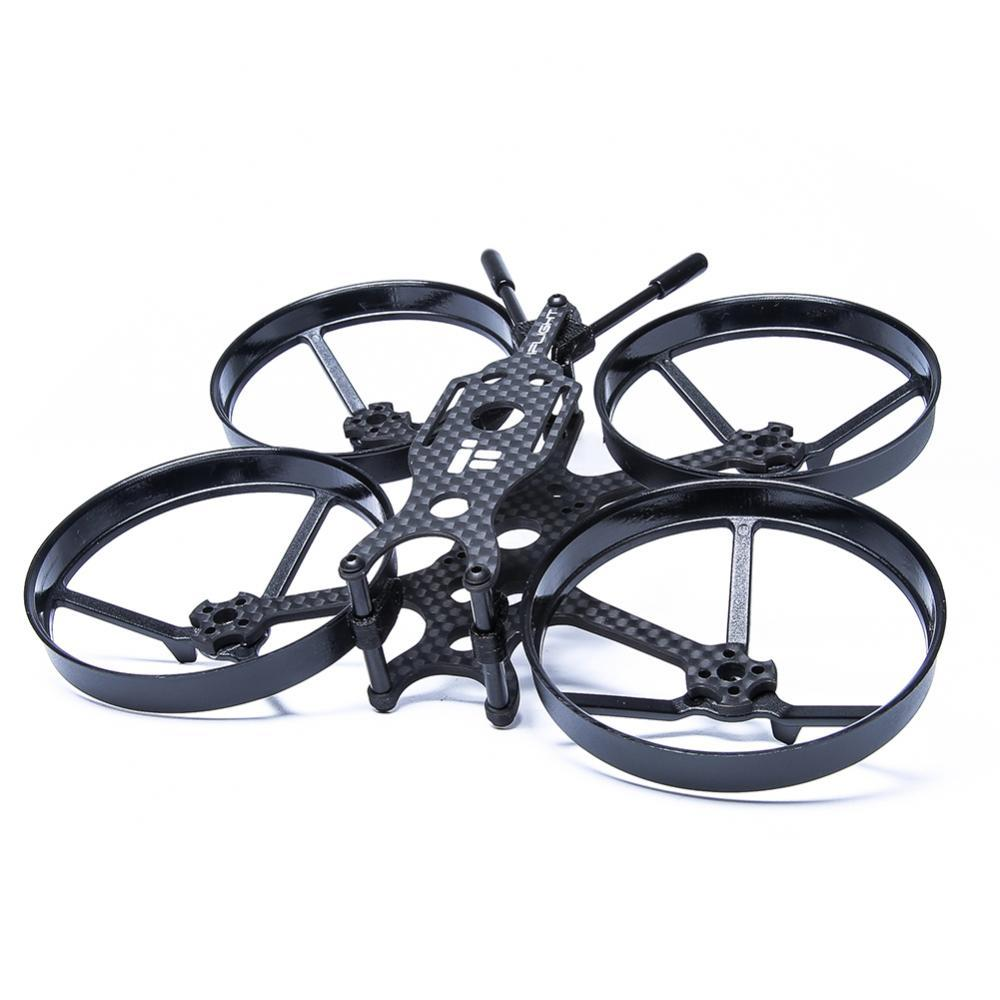
\includegraphics[width=0.5\linewidth]{pics/frame}
	\caption{Рама для экспериментального образца квадрокоптера
	}
	\label{fig:frame} % эта метка позволяет ссылаться на рисунок в тексте
\end{figure}

Электроника квадрокоптера должна быть совместимой по характеристикам и габаритам. 

Для управления с наземной станции полетный контроллер должен:

--- обладать минимум 3 UART портами,

--- иметь процессор на базе F405 / F745 / F765 чипа

UART (Universal asynchronous receiver/transmitter) -- это аппаратный последовательный интерфейс, который позволяет подключать датчики и периферию к полетному контроллеру. У него есть два вывода для внешнего соединения: TX -- для передачи данных, RX -- для приема.

Выбор чипа процессора основан на количестве ресурсов. Для того, чтобы прошить PX4, необходим объем памяти процессора не ниже 1 МБ. Такое условие выполняют процессоры на базе F405 / F745 / F765.
% дописать
Винто-моторная группа должна быть оптимизирована под задачи автономного полета в помещении на небольшой скорости и вмещаться в выбранную раму. У бесколлекторных моторов основными параметрами являются размеры статора, неподвижной части мотора, (4 цифры) и количество оборотов на вольт(kv). В четырех-значном числе первые два отвечают за диаметр статора , вторые -- за высоту статора. При одинаковых объемах статора крутящий момент на низких оборотах будет больше у того мотора, где больше диаметр статора, а на высоких оборотах там, где больше высота. Для экспериментально образца оптимальным выбором являются моторы 1202. Количество оборотов на вольт выберем, учитывая напряжение аккумулятора. Чем больше напряжение, тем меньше количество оборотов на вольт должно быть на моторе. Каждая ячейка, подключенная последовательно увеличивает напряжение на 4.2 В в заряженном состоянии. Для квадрокоптера с диагональю рамы 120 мм по соотношению вес / токоотдача наиболее выгодно ставить аккумуляторы с 2-3 ячейками. Основываясь на таблице характеристик, приведенных производителем, были выбраны моторы с 6000 kv (рис. \ref{fig:motor}).
Учитывая потребление тока моторами на полном газу и добавляя 15 \% запаса, получаем характеристику регуляторов -- максимальный ток, проходящий через них. На экспериментальном образце он равен 15 А.
\begin{figure}[H]
	\centering
	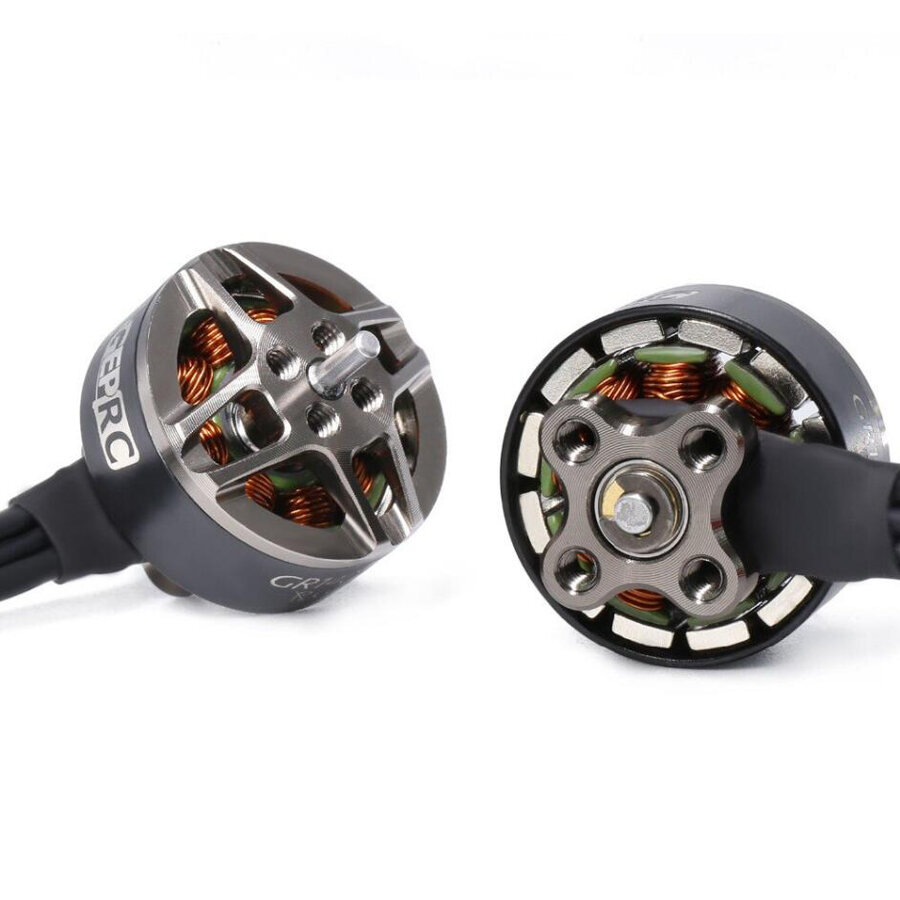
\includegraphics[width=0.5\linewidth]{pics/motor}
	\caption{Моторы для экспериментального образца квадрокоптера
	}
	\label{fig:motor} % эта метка позволяет ссылаться на рисунок в тексте
\end{figure}
\begin{figure}[H]
	\centering
	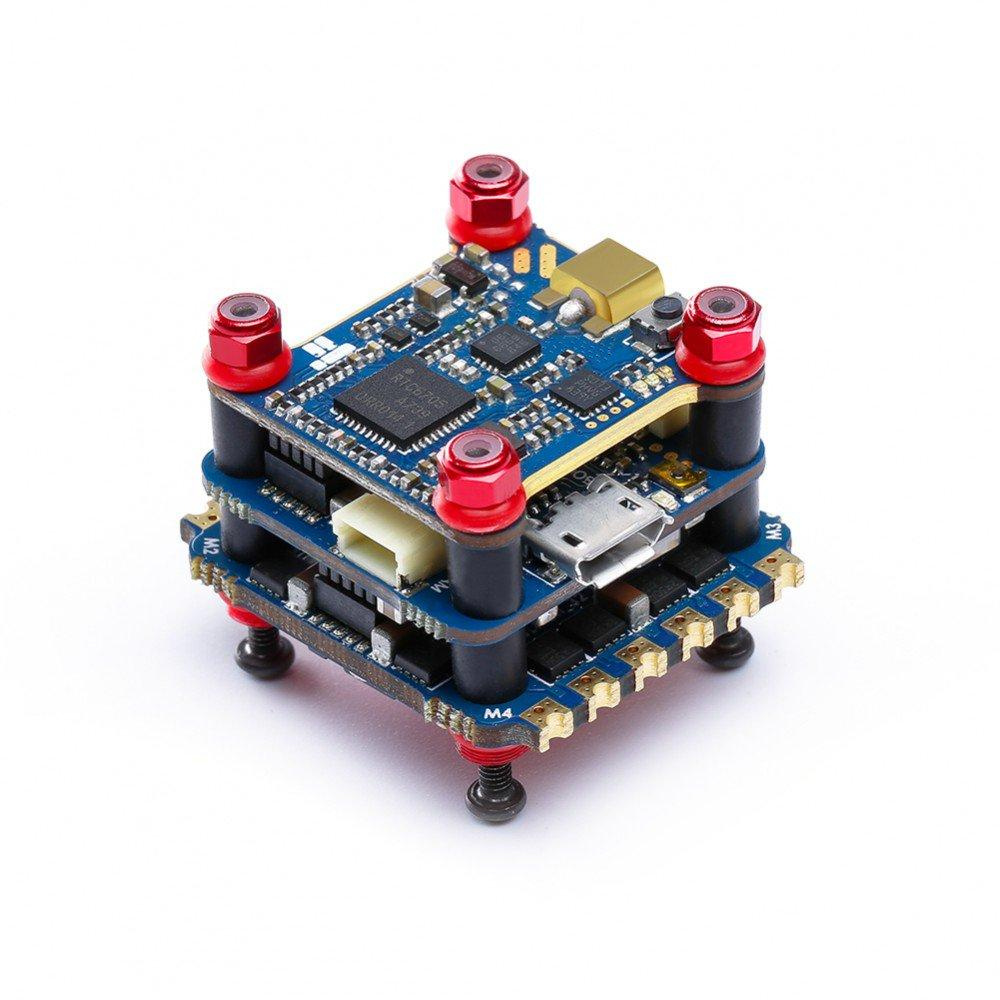
\includegraphics[width=0.5\linewidth]{pics/stack}
	\caption{Стек электроники для экспериментального образца квадрокоптера
	}
	\label{fig:stack} % эта метка позволяет ссылаться на рисунок в тексте
\end{figure}
Видеопередатчик и камера выбирались исходя из поставленных условий. Так как необходимо будет передавать видеопоток, камера должна иметь максимально возможное количество телевизионных линий -- разрешающая способность (TVL). Для камер нано формата это 1000 TVL. Размер изображения может быть как 4:3 и 16:9. Формат PAL / NTSC также может быть выбран на усмотрение.

Видеопередатчик обладает такими характеристиками как:

--- выходная мощность,

--- выходная частота,

--- количество каналов

Для помещений мощность 25mW является оптимальной. Количество каналов должно быть выбрано таким образом, чтобы в случае совместных полетов сигнал не пересекался с сигналом другого беспилотника. Современные видеопередатчики имеют 40 каналов. Частота видеосигнала будет использоваться 5.8ГГц.

Для общения с наземной станцией квадрокоптеру понадобятся устройства приема-передачи телеметрии. Протокол, бауд-рейт и частота устройств станции и квадрокоптера должны совпадать.
% дописать

\subsection{Программная часть}
В качестве прошивки для квадрокоптера был выбран PX4 - проект с открытым исходным кодом, позволяющий выполнять автономные полеты.

%//почему был выбран рх4?

%//его возможности?

%//estimator lpe / ekf
%\url{https://dev.px4.io/v1.9.0/en/ros/offboard\_control.html}
%\url{https://dev.px4.io/v1.9.0/en/ros/external_position_estimation.html}
